% generated by scripts/pkl_to_latex.py
% source PKL : uscan_v1_L6_Ne6_t0p1_mode-uniform_nmin2_solver-gcg_full_es_restarts10_iter300_kmax5_tol1em09_U0.1to5_N21-8081b758e7cc.pkl
% scan type  : uscan
% state      : ex_singlet
% quantity   : vn-entropy
% requires   : \usepackage{pgfplots} \pgfplotsset{compat=1.18}
% colours match the matplotlib PDF (tab10 cycle)
\definecolor{gmeC0}{HTML}{1F77B4}
\definecolor{gmeC1}{HTML}{FF7F0E}
\definecolor{gmeC2}{HTML}{2CA02C}
\definecolor{gmeC3}{HTML}{D62728}
\definecolor{gmeC4}{HTML}{9467BD}
\definecolor{gmeC5}{HTML}{8C564B}
\definecolor{gmeC6}{HTML}{E377C2}
\definecolor{gmeC7}{HTML}{17BECF}

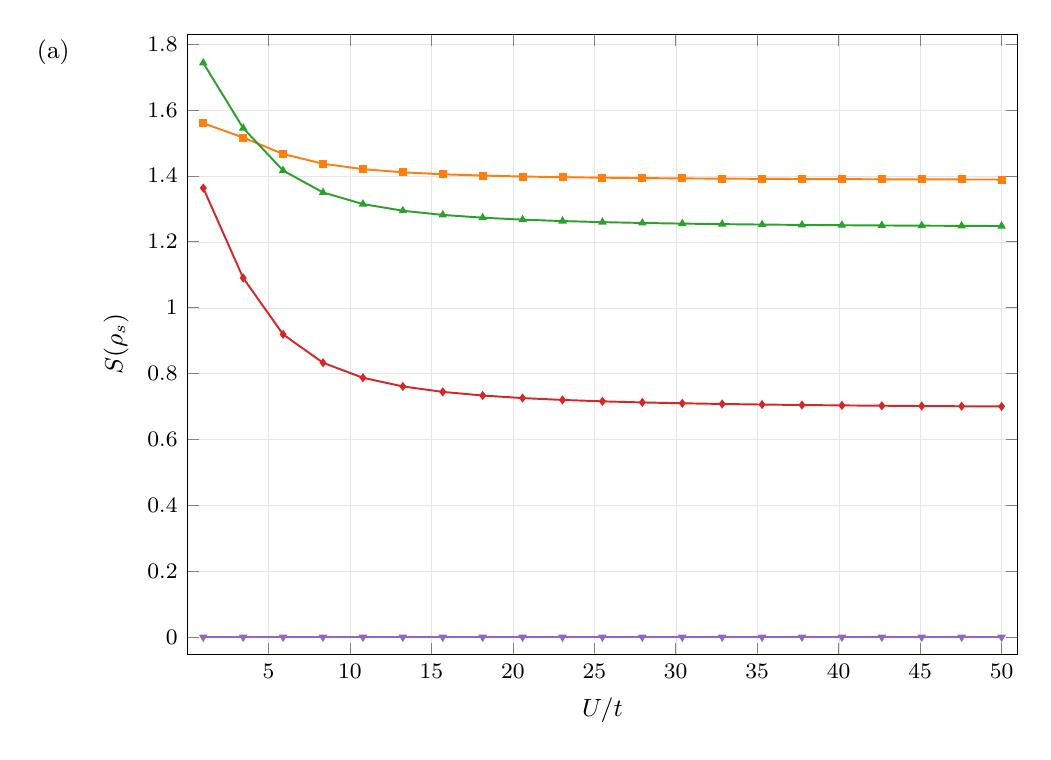
\begin{tikzpicture}
  \begin{axis}[
    width=\columnwidth,
    height=0.78\columnwidth,
    xlabel={$U/t$},
    ylabel={$S(\rho_s)$},
    grid=both,
    grid style={line width=.1pt, draw=gray!20},
    tick label style={font=\footnotesize\rmfamily, /pgf/number format/fixed},
    label style={font=\small\rmfamily},
    scaled ticks=false,
    legend style={font=\scriptsize\rmfamily, draw=gray!40, at={(0.5,1.03)}, anchor=south, /tikz/every even column/.append style={column sep=6pt}},
    legend cell align={left},
    legend columns=2,
    ymin=-0.052,
    ymax=1.83,
    xmin=0.02,
    xmax=50.98,
    after end axis/.append code={\node[anchor=east, font=\small\rmfamily] at (axis description cs:-0.13,0.970) {(a)};},
  ]
    \addplot[color=gmeC1, mark=square*, mark size=1.1pt, line width=0.7pt] coordinates {
        (1,1.559401) (3.45,1.516288) (5.9,1.466226) (8.35,1.436639)
        (10.8,1.420322) (13.25,1.410766) (15.7,1.404758) (18.15,1.400747)
        (20.6,1.397936) (23.05,1.395887) (25.5,1.394347) (27.95,1.393158)
        (30.4,1.39222) (32.85,1.391467) (35.3,1.390852) (37.75,1.390343)
        (40.2,1.389917) (42.65,1.389557) (45.1,1.389249) (47.55,1.388984)
        (50,1.388754)
    };
    \addplot[color=gmeC2, mark=triangle*, mark size=1.1pt, line width=0.7pt] coordinates {
        (1,1.742634) (3.45,1.544796) (5.9,1.416085) (8.35,1.34955)
        (10.8,1.314355) (13.25,1.294065) (15.7,1.281391) (18.15,1.272951)
        (20.6,1.26704) (23.05,1.262733) (25.5,1.259493) (27.95,1.256991)
        (30.4,1.255016) (32.85,1.253428) (35.3,1.252131) (37.75,1.251057)
        (40.2,1.250157) (42.65,1.249395) (45.1,1.248744) (47.55,1.248183)
        (50,1.247695)
    };
    \addplot[color=gmeC3, mark=diamond*, mark size=1.1pt, line width=0.7pt] coordinates {
        (1,1.362758) (3.45,1.090043) (5.9,0.918859) (8.35,0.832693)
        (10.8,0.787214) (13.25,0.760892) (15.7,0.74438) (18.15,0.733344)
        (20.6,0.725595) (23.05,0.719937) (25.5,0.715674) (27.95,0.712377)
        (30.4,0.709772) (32.85,0.707677) (35.3,0.705963) (37.75,0.704544)
        (40.2,0.703354) (42.65,0.702347) (45.1,0.701485) (47.55,0.700742)
        (50,0.700097)
    };
    \addplot[color=gmeC4, mark=triangle*, mark size=1.1pt, mark options={rotate=180}, line width=0.7pt] coordinates {
        (1,0) (3.45,0) (5.9,0) (8.35,0)
        (10.8,0) (13.25,0) (15.7,0) (18.15,0)
        (20.6,0) (23.05,0) (25.5,0) (27.95,0)
        (30.4,0) (32.85,0) (35.3,0) (37.75,0)
        (40.2,0) (42.65,0) (45.1,0) (47.55,0)
        (50,0)
    };
  \end{axis}
\end{tikzpicture}
